\documentclass[aspectration=1610,t]{beamer}
\usepackage{csc}
\title{Лекция 4. OpenGL --- направленное освещение}


\date{
   \textbf{ИТМО}\\
   5 октября 2022\\
   Санкт-Петербург
}

\begin{document}

\begin{frame}
  \titlepage
\end{frame}

\begin{frame}[fragile]{Модель Фонга}
    Одна из самых простых моделей - {\bf модель Фонга}. Состоит из 3 компонент:
    \begin{itemize}
        \item {\bf ambient} - фоновое освещение;
        \item {\bf diffuse} - направленный свет;
        \item {\bf specular} - блик.
    \end{itemize}
    \begin{figure}[htp]
        \centering
        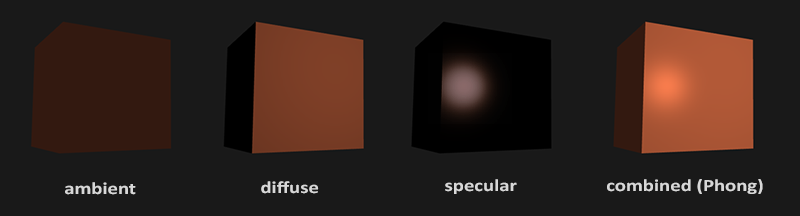
\includegraphics[scale=0.40]{res/phong}
    \end{figure}
\end{frame}

\begin{frame}[fragile]{Ambient}
    Фоновый компонент можно расчитывать следущий образом:
            {\small \begin{lstlisting}
float ambient_strength = 0.1f;
vec3 ambient = ambient_strength * light_color;

vec3 result = ambient * object_color;
color = vec4(result, 1.0f);
            \end{lstlisting}}
\end{frame}

\begin{frame}[fragile]{Diffuse}
    Направленный компонент можно расчитывать следущий образом:
            {\small \begin{lstlisting}
out vec3 frag_pos;  
out vec3 normal;

gl_Position = mvp * vec4(position, 1.0f);
frag_pos = vec3(model * vec4(position, 1.0f));
normal = normal;
            \end{lstlisting}}
\end{frame}

\begin{frame}[fragile]{Diffuse}
    Направленный компонент можно расчитывать следущий образом:
            {\small \begin{lstlisting}
in vec3 normal;  
in vec3 frag_pos;  
    
uniform vec3 light_pos; 
uniform vec3 light_color;
uniform vec3 object_color;

vec3 norm = normalize(normal);
vec3 light_dir = normalize(light_pos - frag_pos);
float diff = max(dot(norm, light_dir), 0.0);
vec3 diffuse = diff * light_color;
            \end{lstlisting}}
\end{frame}

\begin{frame}[fragile]{Нормали}
    При работе с объектами нормали могут измениться:
    \begin{figure}[htp]
        \centering
        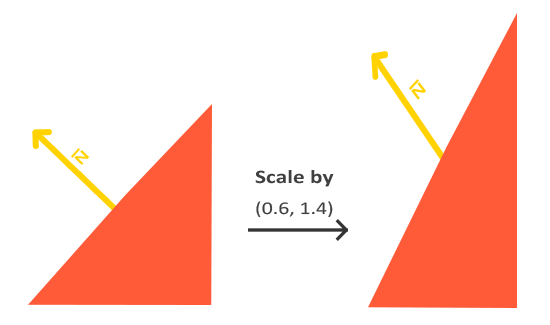
\includegraphics[scale=0.30]{res/norm}
    \end{figure}
    Чтобы сохранить нормали при изменении геометрии используют матрицу нормалей:
    {\small \begin{lstlisting}
normal = mat3(transpose(inverse(model))) * normal;
    \end{lstlisting}}
\end{frame}

\begin{frame}[fragile]{Specular}
    Учитываем только направление источника:
    \begin{figure}[htp]
        \centering
        
\includegraphics[scale=0.2]{res/diff}
    \end{figure}
    Учитываем положение наблюдателя:
    \begin{figure}[htp]
        \centering
        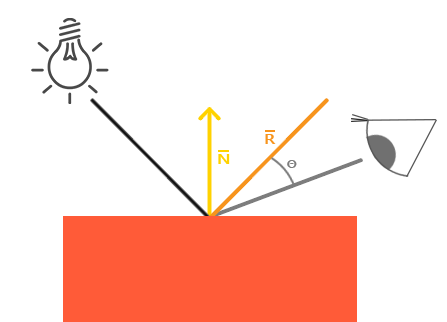
\includegraphics[scale=0.2]{res/spec}
    \end{figure}
\end{frame}

\begin{frame}[fragile]{Specular}
    Компонента для блика:
            {\small \begin{lstlisting}
uniform vec3 view_pos;

float specular_strength = 0.5f;
vec3 viewDir = normalize(view_pos - frag_pos);
vec3 reflect_dir = reflect(-light_dir, norm);  
float spec = pow(
    max(dot(view_dir, reflect_dir), 0.0),
    32);
vec3 specular = specular_strength * spec * light_color; 
            \end{lstlisting}}
\end{frame}

\end{document}

